\documentclass{article}
\usepackage[utf8]{inputenc}
\usepackage[T1]{fontenc}
\usepackage{graphicx}
\usepackage{hyperref}
\usepackage{geometry}
\geometry{margin=1in}

\title{Engraved Plate (Row 251)}
\date{Encyclopaedia Britannica (1771)}

\begin{document}
\maketitle

\section*{Historical source}
\textbf{Entry ID:} \texttt{entry-swooning-251} \\
\textbf{Volume ID:} 191679021 \\
\textbf{Character Count:} 313

\subsection*{Extracted Text}
SWOONING. See Manchiss, n° 273.

[HISTORICAL COPPERPLATE ENGRAVING: Engraved Plate (Row 251)]
Category: Historical Illustration
Visual Description: Historical copperplate engraving from Encyclopaedia Britannica (1771).
Identified Engraved Figures:

Related Scientific Subjects: Encyclopaedia Britannica, Engraving



\section*{Source record}
\begin{itemize}
\item \textbf{Dataset:} \texttt{NationalLibraryOfScotland/encyclopaedia\_britannica\_illustrated}
\item \textbf{Dataset Revision:} \texttt{309f765b1ecc83e0a7f7762e44b4a927a7555443}
\item \textbf{Page ID:} \texttt{britannica:309f765b1ecc83e0a7f7762e44b4a927a7555443:train:251} \\
  \textbf{Filename:} \texttt{page-0251-69952e7c4a0f.jpg} \\
  \textbf{Row Index:} 251 \\
  \textbf{SHA256:} \texttt{69952e7c4a0f4026...}
\end{itemize}

\begin{figure}[h]
\centering
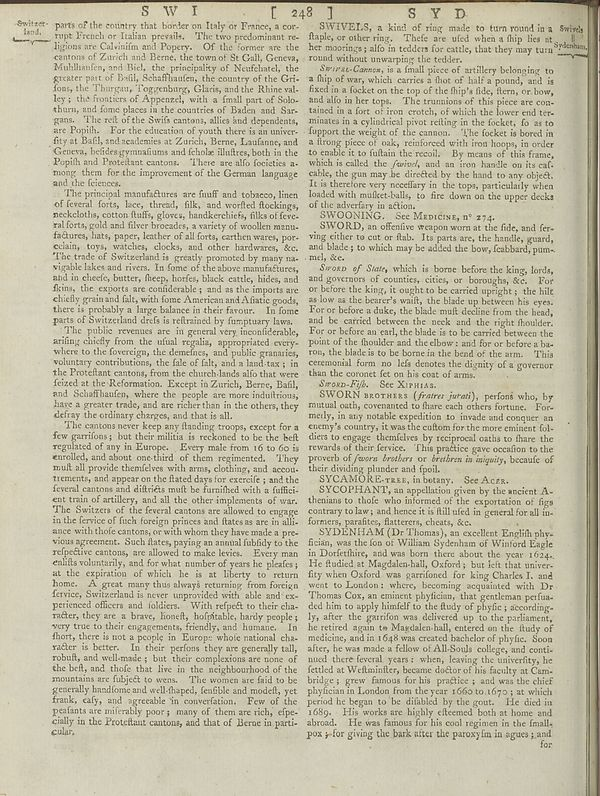
\includegraphics[width=0.85\textwidth]{../scans/page-0251-69952e7c4a0f.jpg}
\caption*{Source scan: \texttt{page-0251-69952e7c4a0f.jpg}}
\end{figure}

\end{document}
